\documentclass[english,version-2022-01]{uzl-thesis} %version-2020-11

\UzLThesisSetup{
  Logo-Dateiname        = {Logo_IMI_de.png},
  Verfasst              = {am}{Institut für Medizinische Informatik},
  Titel auf Deutsch     = {MRT-Registration}, 
  Titel auf Englisch    = {MRT-Registration},
  Autor                 = {Jan Meyer},
  Betreuerin            = {Prof. Dr. Mattias Heinrich},
  Mit Unterstützung von = {Ziad Al-Haj Hemidi, Eytan Kats},
  Masterarbeit,
  Studiengang           = {Medizinische Informatik},
  Datum                 = {1. Januar 2025},
  Abstract              = {Something about MRI and registration},
  Zusammenfassung       = {Irgendwas über MRT und Registration},
  Acknowledgements      = {Danke an Mattias, Ziad und Eytan für die gute Betreuung.},
  Numerische Bibliographie %Alphabetische
}


% Designs
%\UzLStyle{computer modern oldschool design}
%\UzLStyle{computer modern scholary design}
%\UzLStyle{pagella basic design}
%\UzLStyle{pagella centered design}
%\UzLStyle{pagella contrast design}
%\UzLStyle{alegrya basic design}
%\UzLStyle{alegrya scholary design}
%\UzLStyle{alegrya stylish design}
\UzLStyle{alegrya modern design}




%%%%%%%%
%
% Now, include the package you need here using \usepackage. 
%
% However, many standard packages are already loaded by the class:
% amsmath, amssymb, amsthm, babel, biblatex, csquotes, etoolbox,
% filecontents, fontspec, geometry, hyperref, tikz (with libraries
% arrows.meta, positioning and shapes), varioref, url 
%
%%%%%%%
\usepackage{subcaption}	% for subfigures
\usepackage{float}


% add bibliography
%\addbibresource{Bibliography.bib}
\bibliography{Bibliography.bib}


\begin{document}

%%%%%%%%%%%%%%%%%%%%%%%%%
%%%%%  Introduction %%%%%
%%%%%%%%%%%%%%%%%%%%%%%%%

\chapter{Introduction}
Introduction of stuff.

\section{Contributions of the Thesis}
We implemented stuff.

\section{Related Work}
There are many papers on image registration in general, however in the context of medical image registration with deep learning their number is reduced due to the specialized nature of the subject at hand. Yet, there are a couple of papers that give a good overview of the topic.
They give a brief overview of registration methods, basics of deep learning with already existing networks for image registration as well as covering potential applications and challenges~\cite{Chen2020,Haskins2020,Fu2020,Zou2022,Chen2023}.
A lot of different approaches for medical image registration are based on \emph{VoxelMorph}~\cite{Voxelmorph}, such as both \emph{Fourier-Net}~\cite{Fourier-Net} and its successor \emph{Fourier-Net+}~\cite{Fourier-Net+}.


\section{Structure of the Thesis}
This Thesis contains a lot of stuff in different chapters.

%%%%%%%%%%%%%%%%%%%%%%%
%%%%%%%  Basics %%%%%%%
%%%%%%%%%%%%%%%%%%%%%%%

\chapter{Basics}
In this chapter the basics of the thesis are explained.

\section{Magnetic Particle Imaging}
Here MRI is described. % TODO: define abbreviations for CT and MRI here!!

\section{Image Registration}
Image registration is a challenging, yet important task for image processing. It can be described as the process of transforming different image datasets into one coordinate system with matched imaging contents~\cite{Haskins2020}. In the medical field this can be used for clinical applications such as disease diagnosis and monitoring, image-guided treatment delivery, and post-operative assessment. Medical image registration is typically used to pre-process data for tasks like object detection (for e.g. tumor growth monitoring) and segmentation (for e.g. organ atlas creation) where variation in spatial resolution is common between modalities like CT and MRI and patients. Thus the performance of these methods is dependent on the quality of image registration~\cite{Chen2020}. \\
Medical image registration was often done manually by clinicians, however, registration tasks are often challenging and the quality of manual alignments is dependent on the expertise of the user. These manual registrations are thus not only time consuming, but also hardly reproducible leading to high interobserver-variability. The need for automatic registration is very much apparent, but this task remained hard to solve for a long time, requiring a lot of computational power and time for computer algorithms to solve the problem. While neural networks also require a lot of computational power and time to train, they promise fast execution after training. With the rise of deep learning these network gained popularity and now pose a real alternative to conventional algorithms and manual registration~\cite{Haskins2020}. We will discuss these new approaches in the next section, but first we need to formally define our problem.\\
In pair-wise image registration two images ($F$ and $M$) are to be aligned, with $F$ denoting the fixed and $M$ the moving image. T is the desired spatial transformation that aligns the two images. This can be posed as an optimization problem:
\begin{equation}
	T' = \arg\max S(F, T(M)),
\end{equation}
with $T'$ being the best transformation that maximizes the similarity $S$ between the two images. This process is done iteratively improving estimates for the desired T, such that the defined similarity in the cost function is maximized~\cite{Chen2020}.\\
Transformations can be categorized as rigid, affine, and deformable. A rigid transformation consists of rotation and translation; an affine transformation
includes translations, rotations, scaling, and sheering; the two kinds of transformations are described as a 2D single matrix. Unlike rigid and affine transformation, deformable transformation is a high-dimension problem that we need to formulate by a 3D matrix for 2D deformable registration i.e., a so-called deformation field. While rigid and affine registration algorithms have already achieved good performance in many applications, deformable registration is still a challenging task due to its intrinsic complexity, particularly when the deformation is large. However, these are also the transformations most likely encountered in clinical practice as it can be utilized to fuse information from different modalities such as MRI and CT~\cite{Zou2022}. Additionally, deformable image registration can also be
utilized for various computer-assisted interventions like biopsy~\cite{Tam2016} and (MRI-guided) radiotherapy~\cite{Chen2017, Rigaud2019}. \\
Intuitively, deformable image registration is an ill-posed problem, making it fundamentally different from other computer vision tasks such as object localization, segmentation or classification. Given two images, deformable image registration aims to find a spatial transformation that warps the moving image to match the fixed image as closely as possible. However, there is no ground-truth available for the desired deformation field and without enforcing any constraints on the properties of the spatial transformation, the resulting cost function is ill-conditioned and highly non-convex. In order to address the latter and ensure tractability, all image registration algorithms regularize the estimated deformation field, based on some prior assumptions on the properties of the underlying unknown deformation~\cite{Chen2020}.\\
Many methods have been proposed for medical image registration to deal with the complex challenges of this task. Popular conventional registration methods include optical flow~\cite{Yang2008}, demons~\cite{Vercauteren2009} and many more. However, most of these still lack accuracy and computation speed, which makes newer deep learning approaches all the more interesting~\cite{Fu2020}.

\section{Deep Learning Architectures}
Neural networks, despite the theoretical concepts being around for decades, have seen a meteoric rise in popularity over the last few years as constraints on computational power have been alleviated. Especially deep neural networks, which are often summarized under the term deep learning (DL). Recent years have witnessed an almost exponential growth in the development and use of DL algorithms, sustained thus far by rapid improvements in computational hardware (e.g. GPUs). Consequently, clinical applications requiring image classification, segmentation, registration, or object detection/localization, have witnessed significant improvements in algorithmic performance, in terms of accuracy and/or efficiency~\cite{Chen2020}. The following network architecture are widely used for different tasks including medical image registration. \\
Some basic stuff about network training, testing and different architectures that are relevant for the later Chapters.

\subsection{Convolutional Neural Networks}
Convolutional neural networks (CNNs) are a type of deep neural networks with regularized multilayer perceptron, which are mainly used for image processing. CNNs use convolution operations instead of general matrix multiplications in typical neural networks. These convolutional filters make CNNs very suitable for visual signal processing. Because of their excellent feature extraction ability, CNNs are some of the most successful models for image analysis. Different variants of CNN have been proposed and have achieved the-state-of-art performances in various image processing tasks. A typical CNN usually consists of multiple convolutional layers, max pooling layers, batch normalization layers, sometimes dropout layers, a sigmoid or softmax layer. In each convolutional layer, multiple channels of feature maps are extracted by sliding trainable convolutional kernels across the input feature maps. Hierarchical features with high-level abstraction are extracted using multiple convolutional layers. These feature maps usually go through multiple fully connected layer before reaching the final decision layer. Max pooling layers are often used to reduce the image sizes and to promote spatial invariance of the network. Batch normalization is used to reduce internal covariate shift among the training samples. Weight regularization and dropout layers are used to alleviate data overfitting~\cite{Fu2020}. The loss function is often defined as the difference between the predicted and the target output. CNNs are usually trained by minimizing the loss via gradient back propagation using optimization methods like Adam~\cite{Adam}. 
% Convolutions and Deconvolutions genauer erklären?!

\subsection{U-Net}
The U-Net~\cite{U-Net} architecture is an extension of the typical CNNs structure typically used for image segmentation, however it can also be used for image registration tasks. It adopts symmetrical contractive and expansive paths with skip connections between them. The encoding blocks on the left extract important features from the image using convolution layers and max pooling, which are then stored in the latent space in the middle. From there it is reconstructed using upsampling and convolutions in the decoding blocks on the right. Additionally, skip connections are used to improve the spatial resolution of the segmentation. This architecture allows effective feature learning from a small number of training datasets~\cite{Fu2020}. 

\subsection{Autoencoders}
An autoencoder (AE) is a type of CNNs that learns to reconstruct an image from its input without supervision. AEs usually consists of an encoder which extracts the input features, which are stored a low-dimensional latent state space, similar to a U-Net, and a decoder which restore the original input from the latent space. To prevent an AE from learning an identity function, regularized autoencoders were invented, which can be used for e.g. denoising AEs. Variational AEs (VAEs) are generative models that learn latent representation using a variational approach, which constrains the variability of the outputs. VAEs can been used for anomaly detection and image generation~\cite{Fu2020}.

\subsection{Generative Adversarial Networks}
Generative adversarial networks (GANs) consist of two competing networks, a generator and a discriminator. The generator is trained to generate artificial data that approximate a target data distribution from a low-dimensional latent space similar to an AE. The discriminator is trained to distinguish the artificial data from actual data. The discriminator encourages the generator to predict realistic data by penalizing unrealistic predictions via learning. Therefore, the discriminative loss could be considered as a dynamic network-based loss term. The generator and discriminator both are getting better during training to reach Nash equilibrium. In medical imaging, GANs have been used to perform image synthesis for inter- or intra-modality, such as MRI to synthetic CT and vise versa. In medical image registration, GANs are usually used to either provide additional regularization or translate multi-modal registration to uni-modal registration~\cite{Fu2020}.

\section{Deep Learning for Image Registration}
Recently, there has been a surge in the use of deep learning based approaches for medical image registration. Their success is largely due to their ability to perform fast inference, and the flexibility to leverage auxiliary information such as anatomical masks as part of the training process. The most effective methods, such as \emph{VoxelMorph}~\cite{Voxelmorph}, typically employ a U-Net style architecture to estimate dense spatial deformation fields. These methods require only one forward pass during inference, making them orders of magnitude faster than traditional iterative methods. Following the success of \emph{VoxelMorph}, numerous deep neural networks have been proposed for various registration tasks~\cite{Fourier-Net+}. Other approaches also utilize CNNs, AEs and GANs. Typical strategies are discussed in more detail in the following sections.

\subsection{Supervised Registration}
Supervised registration describes training a network with a ground truth displacement field that is either real (created by hand) or synthetic (generated via traditional iterative registration algorithms). Thus the loss can easily be calculated as the difference in the displacement fields of the network prediction and the ground truth. These methods have achieved notable results with real displacement fields as supervision. However, this approach is very limited by the size and the diversity of the dataset. As the displacement fields are often calculated by conventional algorithms their effectiveness might be limited for difficult problems with which the traditional algorithms struggle. Fully supervised methods are widely studied and have notable results, but the generation of real or synthetic displacement fields is hard, and these displacements fields might be different from the real ground truth, which can impact the accuracy and efficiency of these kinds of methods~\cite{Zou2022}. Notable approaches include \emph{BIRNet}~\cite{BIRNet}.

\subsection{Unsupervised Registration}
As the preparation of the ground truth displacement field for supervised methods is inconvenient, limitations in generalizing results in different domains and various registration tasks are inevitable. Thus, unsupervised registration has a more convenient training process with paired images as inputs, but without a ground truth. Generally, unsupervised learning consists of similarity-based and GAN-based methods, where the loss function computes the similarity between the aligned images and the smoothness of the displacement field, rather than the difference to a ground truth~\cite{Zou2022}. Well known example are \emph{IC-Net}~\cite{IC-Net},  \emph{VoxelMorph}~\cite{Voxelmorph}, \emph{TransMorph}~\cite{TransMorph} and \emph{SYMNet}~\cite{SYM-Net}.


\section{MRI Image Reconstruction}
Patient motion during acquisition is one of the major impediments of high-quality MRI scans. This is especially true for thoracic and abdominal imaging, as organs move during breathing. This motion can induce several consequences on MR signal formation. Intraview and interview motion have to be distinguished between: motion is intraview when occurring during individual MR experiments (between RF excitation and echo formation), whereas motion is interview when occurring between individual MR experiments. Whenever the period of motion is slow compared to the period of MR acquisition defined by the repetition time $TR$, the assumption can be made that motion is interview. This is often a reasonable assumption when considering pseudo-periodic motion induced by respiration, and also possibly by cardiac contraction, which are the two common sources of motion in cardiac and abdominal imaging (typically, the adult respiratory period is about 4–5 $s$, and $TR \approx 10 ms$ for fast imaging). Interview motion results in spatial encoding inconsistencies, and thus in image deterioration which can take complex forms (blurring/ghosting artifacts) as acquisition is performed in a Fourier space. Several strategies can be employed in order to handle patient motion better. Patient cooperation is the most commonly used method. However, breath-holds cannot last much longer than $20 s$ and physiological drifts cannot be completely avoided. This leads to a limitation on the time-period of signal recording and thus, signal-to-noise ratio (SNR). Moreover, the position of organs in successive breath-holds may not be reproducible. Synchronization techniques are well-established and systematically used in clinical protocols, but they require a high-level of motion reproducibility. This is often a limiting factor considering heart rate variability (whether in free breathing or during a breathhold), and respiratory variability in terms of amplitude and frequency. This is why alternative techniques have been put forward with the aim of inverting the process of spatial encoding of moving structures that underlies artifacts. While it is possible to correct for motion prospectively, by modulating the magnetic field gradients and RF fields in order to cancel the effect of motion in the Bloch equations, the method is limited to correcting of, at best, affine motion, due to magnetic field gradient systems being linear. Motion can also be compensated for in reconstruction, however, many methods are restricted to rigid or affine motion due either to computational issues or to the difficulty of modeling complex displacement fields~\cite{GRICS}. The latter however seems to become less of a problem as image registration improves with e.g. the help of deep learning.\\
Motion-resolved data acquisition for these applications are usually accelerated by Parallel Imaging or Compressed Sensing techniques yielding sub-Nyquist sampled (subsampled) k-space data. In order to reconstruct aliasing-free images, these methods rely on reconstruction schemes that, for example incorporate sparsity or low-rank constraints to solve the ill-posed problem. Fixed sparsity assumptions in Compressed Sensing are often too restrictive and incapable of fully modeling spatio-temporal dynamics. Careful fine-tuning between regularization and data consistency is required and especially in highly subsampled cases residual aliasing may remain in the image (under-regularization) or staircasing and blurring artifacts can occur (over-regularization) which affect the image registration. After reconstruction, non-rigid motion fields can be estimated in image space from reconstructed images by solving a registration problem. A particular interest and challenge lies in the derivation of reliable motion fields which capture the spatio-temporal non-rigid deformations, such as respiratory or cardiac movement. Instead of performing these two steps sequentially, motion-compensated image reconstruction schemes like \emph{GRICS}~\cite{GRICS} integrate both motion field estimation and motion correction into the reconstruction process. These methods require reliable motion-resolved images from which the motion fields can be estimated. Motion field estimation can be controlled or supported by external motion surrogate signals, initial motion field estimates, from motion-aliased images or low-frequency image contents. Moreover, spatio-temporal redundancies can be exploited to achieve an aliasing-free image. While these methods have been proven to be more robust against registration errors, they can require a significantly increased computational demand and/or limit imaging acceleration~\cite{Kuestner2022}.

There are also approaches for learning new subsampling strategies in a data-driven manner (pruning unimportant k-space frequencies)~\cite{MRISubsamplingPruning} as well as deep learning based radial~\cite{DeepMRIReconstructionRadialSubsampling} and non-Cartesian~\cite{DeepMRIReconstructionSubsampling} subsampling for MRI acceleration.

%%%%%%%%%%%%%%%%%%%%%%%%
%%%%%  Methodology %%%%%
%%%%%%%%%%%%%%%%%%%%%%%%

%\chapter{Methodology}
%In this chapter the main part of the actual work is discussed.

\chapter{Data}
In the following chapter, the datasets used in this thesis are presented and potential pre-processing steps, as well as uses, discussed. The first dataset \emph{OASIS} containing MRI brain scans was used in the original publications for training and evaluating both \emph{Fourier-Net} and \emph{Fourier-Net+}. It was thus used to get familiar with these networks and their respective work-flows. For our major experiment the \emph{CMRxRecon} dataset was later used. The cardiac MRI data was used for extending the networks to frame-to-frame registration in order for them to be integrated into a motion reconstruction pipeline.

\section{OASIS}
The \emph{OASIS-1} dataset~\cite{OASIS} contains T1-weighted MRI brain scans from 454 subjects and was mainly used for training and testing the original \emph{Fourier-Net/Fourier-Net+}. The brain scans were further pre-processed by~\cite{HyperMorph} for the \emph{Learn2Reg}-Challenge~\cite{Learn2Reg}. This enables subject-to-subject brain registration, as all MRI scans were bias-corrected, skull-stripped, aligned, and cropped to the size of $160 \times 192 \times 224$. The images were stored in the \emph{NIFTI} format,  which makes it really easy to use. Examples can be seen in Figures~\ref{fig:image1} and \ref{fig:image2} with slices from the center of the x-, y- and z-axis.

\begin{figure}[htpb]
	\centering
	\graphicspath{{images/}{\main/images/}}
	\begin{subfigure}{0.45\textwidth}
    		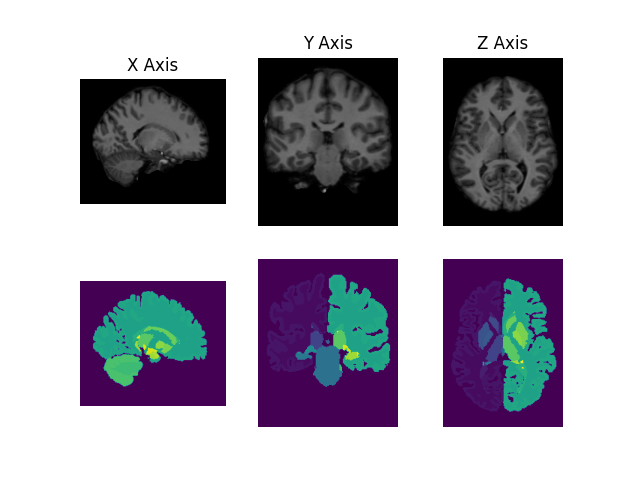
\includegraphics[width=\textwidth]{image2.png}
    		%\caption{Example Image from the Dataset with corresponding labels.}
		\caption{}    		
    		\label{fig:image2}
	\end{subfigure}
	\hfill
	\begin{subfigure}{0.45\textwidth}
    		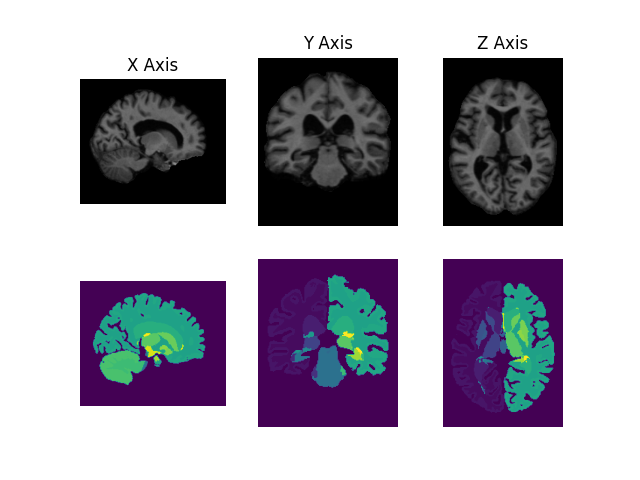
\includegraphics[width=\textwidth]{image1.png}
    		%\caption{Another example Image from the Dataset with corresponding labels.}
		\caption{}    		
    		\label{fig:image1}
	\end{subfigure}
	\caption{Example images (upper row) from the \emph{OASIS} dataset with corresponding labels (bottom row).}
	\label{fig:OASIS}
\end{figure}

\section{CMRxRecon}
The \emph{CMRxRecon} dataset~\cite{CMRxRecon} from the \emph{CMRxRecon2024} challenge specializes in Cardiac magnetic resonance imaging (CMR). The dataset includes multi-contrast k-space data, consisting of cardiac cine, T1/T2-mapping, tagging, phase-contrast (i.e., flow2d), and dark-blood imaging. It also includes imaging of different anatomical views like long-axis (2-chamber, 3-chamber, and 4-chamber), short-axis (SAX), left ventricul outflow tract (LVOT), and aorta (transversal and sagittal views). There is a total of 200 training data, 60 validation data, and 70 test data from healthy volunteers, however the test data is being withheld until the challenge is finished. One of the goals of the challenge is the reconstruction from subsampling and motion correction for the heart movement.

\subsection{Image Reconstruction}
As the data was recorded in the k-space (see Figure~\ref{fig:k-space}) and stored as \emph{.mat} files we first need to reconstruct the images to use them for training and testing of \emph{Fourier-Net/Fourier-Net+}. For this, multi-coil reconstruction algorithms like \emph{SENSE}~\cite{SENSE1} can be used. The sensitivity of the different coils can be seen in Figure~\ref{fig:Coils}, where each coil focuses on a specific area of the image. These images are then stitched together in reconstruction to produce a combined image with great overall contrast.
%, while Figure~\ref{fig:ImageSlice} contains the complete reconstructed image. 
The dataset, as mentioned before, contains fully sampled as well as subsampled k-space data (see Figure~\ref{fig:fullySampled} and Figure~\ref{fig:subSampled}), with the latter being typically used to accelerate the MRI acquisition process. This is done by not using all of the available k-space data, but rather masking the signal to achieve the subsampling. The center region of the k-space is always fully sampled, but the outer regions are subsampled depending on the sampling strategy~\cite{SubsamplingStrategies}. The dataset contains subsampled k-space data for 4x and 8x acceleration with the latter of course leading to more distortions in the reconstructed image as the subsampling can induce image reconstruction artifacts. This can be seen in Figure~\ref{fig:subSampledImage}, where the image reconstructed from 4x accelerated k-space data seems blurred when compared to the fully sampled one in Figure~\ref{fig:fullySampledImage}. 
%An example image can be seen in Figure~\ref{fig:Subsampling} where the k-space of the original image is subsampled with a random mask leading to heavy blurring artifacts after the reconstruction.
For all experiments the short-axis  view data was used. As image sizes between patients can vary slightly, interpolation was used to standardize the images to a size of $246 \times 512$ to avoid further problems with e.g. 
%ensure coherent sizes between images to avoid problems with the network and 
loss calculation. Additionally, min-max-normalization is used to standardize the data range for all images to $[0,1]$ as this was also varying. The reconstructed images were stored for every image slice for every patient. Thus, all frames for a specific image slice were in a single folder to enable easy access for later data load-in for frame-to-frame registration.

\begin{figure}[htpb]
	\centering
	\graphicspath{{images/}{\main/images/}}
	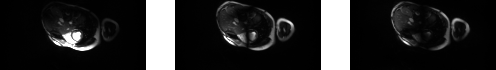
\includegraphics[width=\linewidth]{CoilsHorizontal.png} 
	\caption{MRI images for three different coils from the \emph{CMRxRecon} dataset~\cite{CMRxRecon}.}
	\label{fig:Coils}
\end{figure}


\begin{figure}[htpb]
	\centering
	\graphicspath{{images/}{\main/images/}}
	\begin{subfigure}{0.4\textwidth}
    		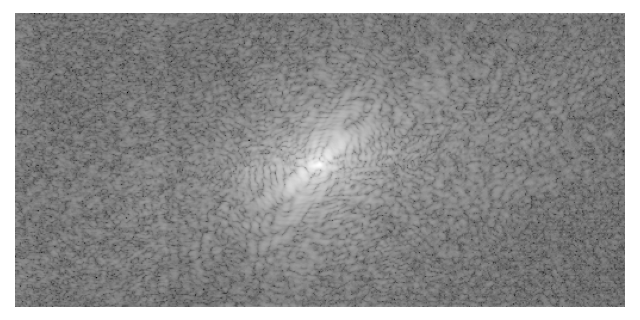
\includegraphics[width=\textwidth]{k-space_fullysampled.png}
    		\caption{Example for a fully sampled k-space.}
    		\label{fig:fullySampled}
	\end{subfigure}
	\hfill
	\begin{subfigure}{0.4\textwidth}
    		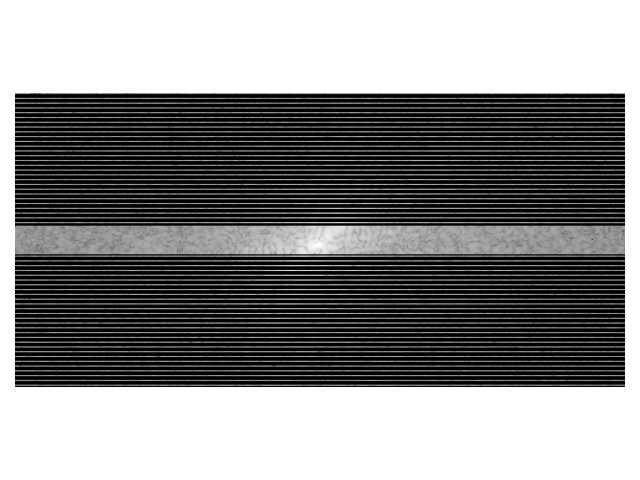
\includegraphics[width=\textwidth]{k-space_subsampled.png}
    		\caption{Example of a subsampled k-space for 4x acceleration.}
    		\label{fig:subSampled}
	\end{subfigure}\\
	\begin{subfigure}{0.4\textwidth}
    		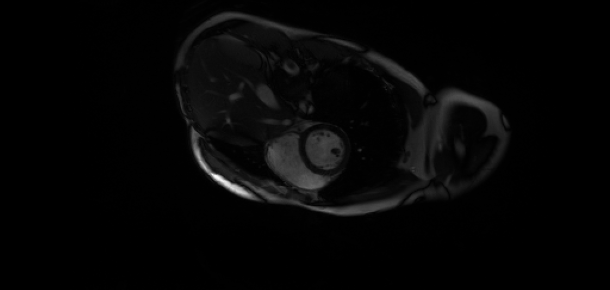
\includegraphics[width=\textwidth]{image_fullysampled.png}
    		\caption{Corresponding image reconstructed from fully sampled k-space.}
    		\label{fig:fullySampledImage}
	\end{subfigure}
	\hfill
	\begin{subfigure}{0.4\textwidth}
    		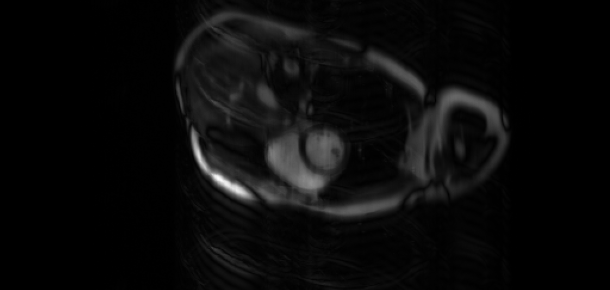
\includegraphics[width=\textwidth]{image_subsampled.png}
    		\caption{Corresponding image reconstructed from subsampled k-space.}
    		\label{fig:subSampledImage}
	\end{subfigure}
	\caption{Fully sampled and subsampled k-space data from the from the \emph{CMRxRecon} dataset~\cite{CMRxRecon} with corresponding images.}
	\label{fig:k-space}
\end{figure}


%\begin{figure}[htpb]
%	\centering
%	\graphicspath{{images/}{\main/images/}}
%	\begin{subfigure}{0.4\textwidth}
%    		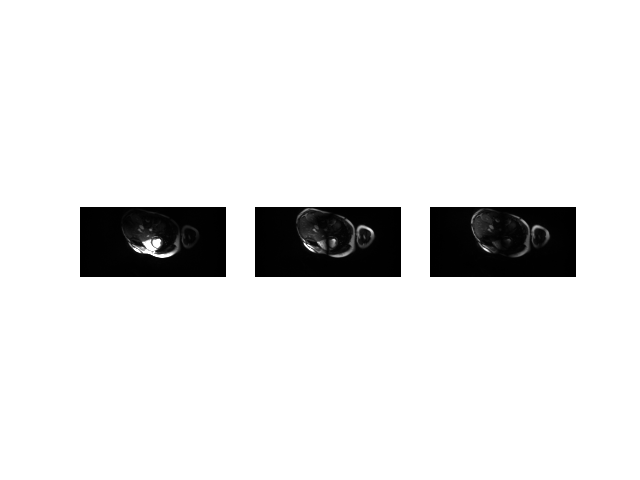
\includegraphics[width=.75\textwidth]{Coils.png}
%    		\caption{MRI images for three different coils.}
%    		\label{fig:Coils}
%	\end{subfigure}
%	\hfill
%	\begin{subfigure}{0.4\textwidth}
%    		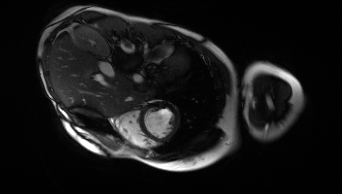
\includegraphics[width=\textwidth]{ImageSlice.png}
%    		\caption{Reconstructed image from the three different coils.}
%    		\label{fig:ImageSlice}
%	\end{subfigure}
%	\caption{Example from the \emph{CMRxRecon} dataset.}
%	\label{fig:CMRxRecon}
%\end{figure}

%\begin{figure}[htpb]
%	\centering
%	\graphicspath{{images/}{\main/images/}}
%	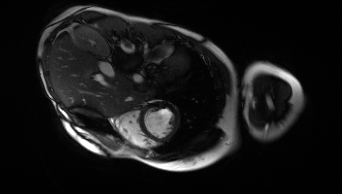
\includegraphics[width=.5\linewidth]{ImageSlice.png} 
%	\caption{Reconstructed image slice from the different coils from the \emph{CMRxRecon} dataset~\cite{CMRxRecon}.}
%	\label{fig:ImageSlice}
%\end{figure}

%\begin{figure}[htpb]
%	\centering
%	\graphicspath{{images/}{\main/images/}}
%	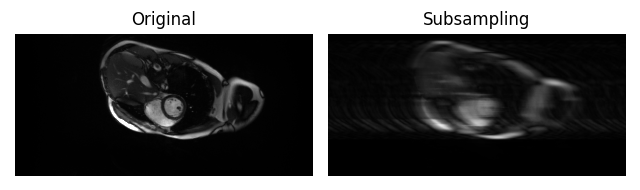
\includegraphics[width=\linewidth]{Subsampling.png} 
%	\caption{Example for blurring artifacts encountered during image reconstruction after subsampling the k-space.}
%	\label{fig:Subsampling}
%\end{figure}

\subsection{Pre-Processing}
As seen before, a large part of the image is just black background that contains no usable information. The interesting cardiac region in the image, however, is much smaller and thus image cropping can be used to extract it. The fairly large image size can thus be cut down without losing important image information, which also helps with memory efficiency. One problem however remains: image alignment. Whereas in the \emph{OASIS} dataset the brain scan were already aligned, the cardiac data in the \emph{CMRxRecon} dataset is not. Thus, one cannot simply center-crop all images as the cardiac region might be located in very different parts of the image. To resolve this issue, adaptive cropping with automatic detection of the cardiac region in the images is needed. \\
To begin, some assumption about the data needs to be made: First, the cardiac region is at the same position for all slices and frames from one patient. Second, most of the movement happens in the cardiac region between frames. From the latter we can conclude that we need to examine the frames, thus the difference between consecutive frames is calculated and averaged for each slice. According to the first assumption this process is repeated for all slices and their results summed to create a sort of heatmap as seen in Figure~\ref{fig:SumDifferences} with a clearly higher intensity in the cardiac region compared to the background. To further isolate this region a simple thresholding is performed followed by an opening operation, which removes any smaller fragments still left in the image. The cardiac region is now clearly separated from the rest of the image as seen in Figure~\ref{fig:MaskCropping}. The only step left is to calculate the approximate center of this region and create a crop around it. To drastically reduce the image size a cropping factor of one third was used, reducing the image size from $246 \times 512$ to $82 \times 170$. The result of this drastic crop can be seen in Figure~\ref{fig:ImageCropped} when compared to the original image in Figure~\ref{fig:fullImage}. Note, however, that the cropped image in Figure~\ref{fig:ImageCropping} appears larger than it actually is, when compared to the original, to allow for a more detailed look. Thus both images are not presented to scale, but in order to show the most image detail.

\begin{figure}[htpb]
	\centering
	\graphicspath{{images/}{\main/images/}}
	\begin{subfigure}{0.6\textwidth}
    		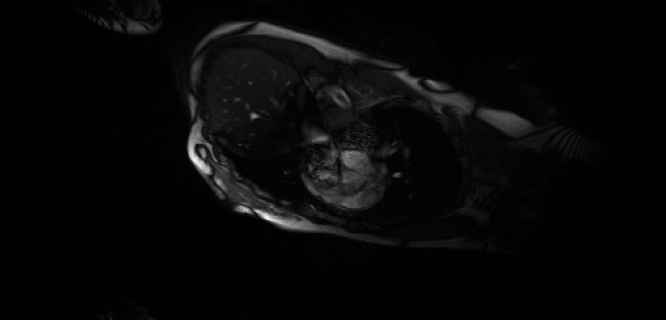
\includegraphics[width=\textwidth]{FullImage.png}
    		\caption{The original full-size image.}
    		\label{fig:fullImage}
	\end{subfigure}
	\\
	\begin{subfigure}{0.6\textwidth}
    		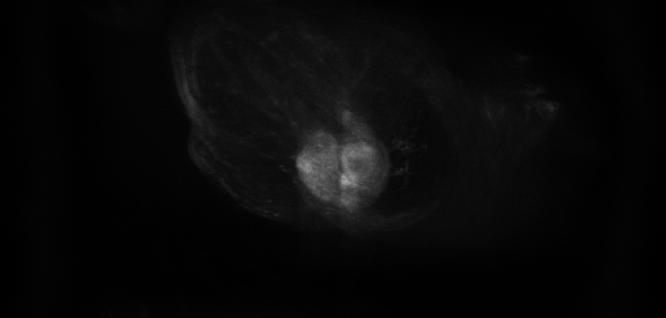
\includegraphics[width=\textwidth]{DifferencesSlices.png}
    		\caption{Sum of the differences between slices and their respective frames with the cardiac region in the middle.}
    		\label{fig:SumDifferences}
	\end{subfigure}
	\\
	\begin{subfigure}{0.6\textwidth}
    		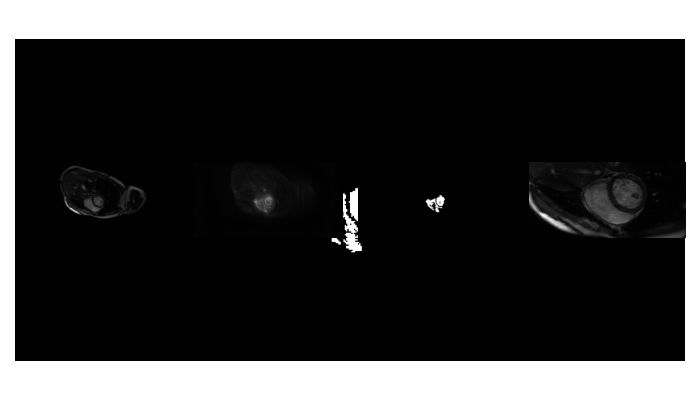
\includegraphics[width=\textwidth]{MaskForCropping.png}
    		\caption{Mask of the cardiac region generated from the sum of differences by thresholding and opening.}
    		\label{fig:MaskCropping}
	\end{subfigure}
	\\
	\begin{subfigure}{0.6\textwidth}
    		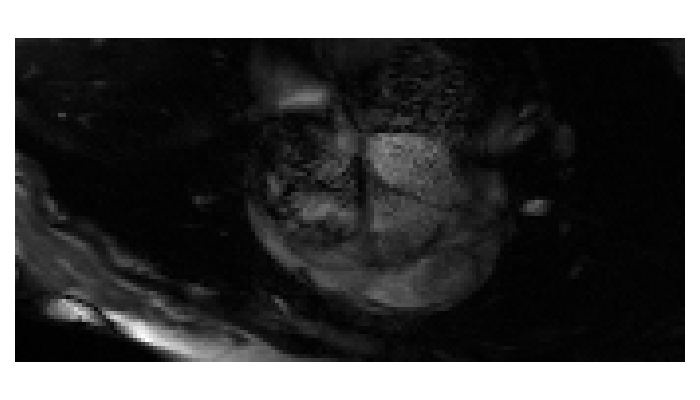
\includegraphics[width=\textwidth]{ImageCrop.png}
    		\caption{The corresponding cropped image.}
    		\label{fig:ImageCropped}
	\end{subfigure}
	\caption{Cropping of an example image by locating the movement between frames for each slice. Note that the cropped image appears larger than it actually is compared to the original.}
	\label{fig:ImageCropping}
\end{figure}

\chapter{Network Architectures}
As a starting point \emph{Fourier-Net}~\cite{Fourier-Net} and its successor \emph{Fourier-Net+}~\cite{Fourier-Net+} were used. These networks, which are explained in the following pages, enable fast and accurate registration while needing less resources compared to similar approaches. These attributes are very beneficial for a potential application like motion correction because the current networks, e.g. \emph{LAPNet}, are usually supervised and require large computational resources.

\section{Fourier-Net}
\emph{Fourier-Net} is a new unsupervised approach that aims to learn a low-dimensional representation of the displacement field in a band-limited Fourier domain instead of the full field in the spatial domain. This band-limited representation is then decoded by a model-driven decoder to the dense, full-resolution displacement field in the spatial domain. This allows for fewer parameters and computational operations, resulting in faster inference speeds~\cite{Fourier-Net}. The architecture is based on the U-Net~\cite{U-Net}, like most deep registration approaches, but replaces the expanding path with a parameter-free model-driven decoder as mentioned before. The encoder of \emph{Fourier-Net} consists of a CNN, which takes two images (fixed and moving) as inputs. The output is a displacement field that is then converted from the spatial domain into the Fourier domain via an discrete Fourier transformation (DFT). From there, this band-limiting representation 
%of the displacement field 
is padded with zeros to the full resolution of the original displacement field. The field is then recovered by using the inverse DFT (iDFT) to convert it back into the spatial domain. This displacement field is then used to warp the moving image into the fixed image. Additionally, squaring and scaling layers~\cite{Dalca2018} can be added before warping the image in order to encourage a diffeomorphism in final deformation. 

\begin{figure}[htpb]
	\centering
	\graphicspath{{images/}{\main/images/}}
	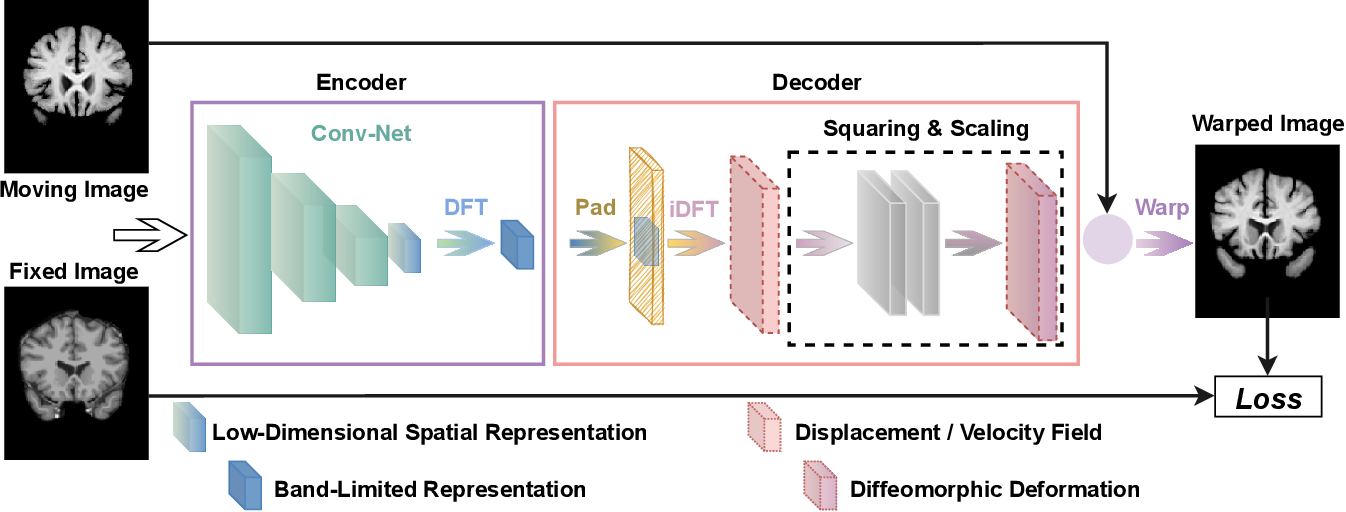
\includegraphics[width=\linewidth]{ArchitectureFourier-Net.png} 
	\caption{Architecture of \emph{Fourier-Net} taken from~\cite{Fourier-Net}.}
	\label{fig:Fourier-Net}
\end{figure}

\subsection{Encoder}
The encoder of \emph{Fourier-Net} consists of a CNN that generates the displacement field between the two inputs followed by a DFT layer that produces a band-limited representation of the full displacement field. The fully convolutional neural network (FCN) from \emph{SYMNet}~\cite{SYM-Net} was modified to function as the CNN of the encoder. Its (original) architecture (see Figure~\ref{fig:SYMNet}) is again based on the \emph{U-Net} with a contracting and expanding path. 
\begin{figure}[htpb]
	\centering
	\graphicspath{{images/}{\main/images/}}
	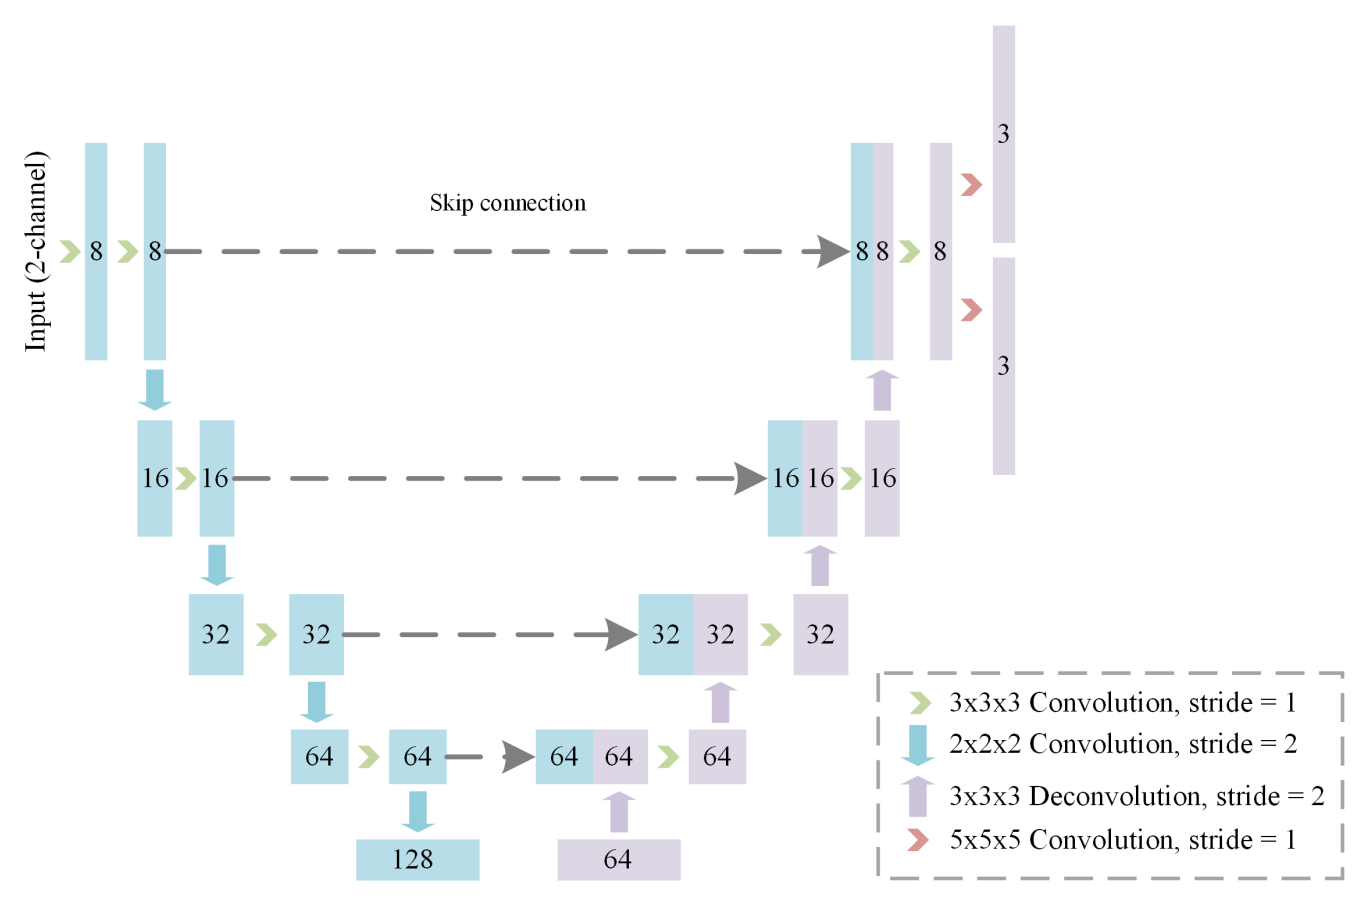
\includegraphics[width=\linewidth]{SYMNetArchitectureFCN.png} 
	\caption{Architecture of the FCN from \emph{SYMNet}~\cite{SYM-Net}.}
	\label{fig:SYMNet}
\end{figure}
The FCN concatenates the inputs images $X$ and $Y$ as a single 2-channel input and estimates two dense, non-linear displacement fields $\phi_{XY}$ and $\phi_{YX}$, however we only need the displacement field for the moving image, denoted as $\mathbb{S}_\phi$, since we are not interested in transforming the fixed image. This is actually a low dimensional representation because \emph{Fourier-Net} does not utilize the last two levels of the FCNs expanding path that would be needed to reconstruct the actual full-resolution displacement field $\phi$.\\
For each level in the contracting path of the FCN, two successive convolution layers are applied, which contain one $3 \times 3 \times 3$ convolution layer with a stride of 1, followed by a $3 \times 3 \times 3$ convolution layer with a stride of 2 to further compute the high-level features between the input images as well as downsample the features by half until the lowest level of the network is reached. For each level in the expanding path of the FCN, the feature maps from the contracting path are concatenated through skip connections and apply $3 \times 3 \times 3$ convolution with a stride of 1 and $2 \times 2 \times 2$ deconvolution layer for upsampling the feature maps to twice of its size. At the end of the expanding path, two $5 \times 5 \times 5$ convolution layers with a stride of 1 are appended to the last convolution layer and generate the displacement fields $\theta_{XY}$ and $\theta_{YX}$~\cite{SYM-Net}. Each convolution layer in the FCN is followed by a rectified linear unit (ReLU) activation, except for the output convolution layer that does not have an activation function because \emph{Fourier-Net} only uses the first two levels of the expanding path, thus leading the FCN to generate a low dimensional representation $\mathbb{S}_\phi$ of the full-resolution displacement field $\phi$.\\
%, where a SoftSign activation function is used~\cite{SYM-Net}:
%\begin{equation}
%	\text{SoftSign}(x) = \frac{x}{1 + |x|} .
%\end{equation}
As discussed previously, the encoder aims to learn a displacement (or velocity) field in the band-limited Fourier domain. Intuitively, this may require convolutions to be able to handle complex-valued numbers, which can be done by using complex-valued CNNs~\cite{Trabelsi2017}, which are suitable when both input and output are complex values, however these complex-valued operations sacrifice computational efficiency. Other approaches like \emph{DeepFlash}~\cite{DeepFlash} tackle this problem by converting the input images to the Fourier domain and using two individual real-valued CNNs to learn the real and imaginary parts separately. This, however, increases training and inference cost. To bridge the domain gap between real-valued spatial images and complex-valued band-limited displacement fields without increasing complexity, \emph{Fourier-Net} uses a DFT layer after the FCN. This is a simple and effective way to produce complex-valued band-limited displacement fields without the network needing to be able to handle complex values itself. The DFT applied to the displacement field $\phi$ can be defined as follows:
\begin{equation} \label{eq:DFT}
	[\mathcal{F}(\phi)]_{k,l} = \sum^{H-1}_{n=0} \sum^{W-1}_{m=0} \phi_{n,m} \cdot \exp \Bigg(i \cdot \bigg(\frac{2 \pi k}{H} \cdot n + \frac{2 \pi l}{W} \cdot m \bigg) \Big),
\end{equation}
where $\phi$ has size $H \times W$, $n \in [0,H-1]$ and $m \in [0,W-1]$ are the discrete indices in the spatial domain, and $k \in [0,H-1]$ and $l \in [0,W-1]$ are the discrete indices in the frequency domain with $i$ being the imaginary unit. However, $\phi$ in this equation is actually the low dimensional representation of the displacement field output by the modified FCN, which can be formulated as follows:
\begin{equation} \label{eq:FCN}
	\mathbb{S}_\phi = \text{FCN}(M,F;\Theta),
\end{equation}
with $M$ being the moving and $F$ the fixed image, as well as $\Theta$ representing the parameters of the FCN. Thus, the whole encoder can be defined 
%mathematically 
as:
\begin{equation}\label{eq:encoder}
	\mathbb{B}_\phi = \mathcal{F}(\mathbb{S}_\phi) = \mathcal{F}(\text{FCN}(M,F;\Theta)),
\end{equation}
with the DFT layer $\mathcal{F}$, full-resolution spatial displacement field $\phi$ and the complex band-limited displacement field $\mathbb{B}_\phi$. The low dimensional representation $\mathbb{S}_\phi$ actually contains all the information of the band-limited Fourier coefficients in $\mathbb{B}_\phi$. As such, \emph{Fourier-Net} does not need to learn the coefficients of $\mathbb{B}_\phi$, but instead only the real-valued coefficients in $\mathbb{S}_\phi$, which is the low dimensional spatial representation of the full-resolution spatial displacement field $\phi$, which is then reconstructed by the decoder. 


\subsection{Decoder}
The decoder contains no learnable parameters, instead the usual expansive path is replaced with a zero-padding layer, an iDFT layer, and an optional squaring and scaling layer. \\
The output from the encoder is a band-limited representation $\mathbb{B}_\phi$ in the frequency domain of the low dimensional displacement field $\mathbb{S}_\phi$ in the spatial domain. To recover the full-resolution displacement field $\phi$ in the spatial domain, we first pad the patch $\mathbb{B}_\phi$, containing mostly low frequency signals, to the original image resolution with zeros. We then feed the zero-padded complex-valued coefficients, denoted as $\mathcal{F}(\phi)$, to an iDFT layer consisting of two steps: shifting the Fourier coefficients from centers to corners and then applying the iDFT to convert them into the spatial domain:
\begin{equation} \label{eq:iDFT}
	\phi_{n,m} = \frac{1}{HW} \sum^{H-1}_{k=0} \sum^{W-1}_{l=0} \mathcal{D}_{k,l} [\mathcal{F}(\phi)]_{k,l} \cdot \exp \Bigg(i \cdot \bigg(\frac{2 \pi n}{H} \cdot k + \frac{2 \pi m}{W} \cdot l \bigg) \Bigg).
\end{equation}
The $H \times W$ sized sampling mask $\mathcal{D}$ is a low-pass filter that has zeros as entries if they are on the positions of high-frequency signals in $\phi$ and ones if they are on the low-frequency positions. Thus we can reconstruct the full spatial displacement field $\phi$ from $\mathbb{B}_\phi$ despite the latter being band-limited. Approaching the problem from the other side we can also think about working backwards from the final displacement. For this, after applying equation~(\ref{eq:DFT}), the low-frequency signals are shifted to a center patch with size $\frac{H}{a} \times \frac{W}{b}$ with $a = 2 \cdot Z_a, b = 2 \cdot Z_b, Z_a, Z_b \in \mathbb{Z}^+$, which is then center-cropped to get $\mathbb{B}_\phi$. This crop of $\mathcal{F}(\phi)$ can be reconstructed using the iDFT from equation~(\ref{eq:iDFT}) with the cropping functioning as a kind of low-pass filtering:
\begin{equation} \label{eq:decoder}
	[\mathbb{S}_\phi]_{n,m} = \frac{ab}{HW} \sum^{\frac{H}{a}-1}_{k=1} \sum^{\frac{W}{b}-1}_{l=1} [\mathbb{B}_\phi]_{k,l} \cdot \exp \Bigg(i \cdot \bigg(\frac{2 \pi a n}{H} \cdot k + \frac{2 \pi b m}{W} \cdot l \bigg) \Bigg),
\end{equation}
with $n \in [0, \frac{H}{a}-1]$ and $m \in [0, \frac{W}{b}-1]$ being the indices of the spatial domain, while $k \in [0, \frac{H}{a}-1]$ and $l \in [0, \frac{W}{b}-1]$ are the indices of the frequency domain with $i$ being the imaginary unit. Thus $\mathbb{S}_\phi$ actually contains all the necessary information from $\phi$, as long as they have the same low-frequency coefficients $\mathbb{B}_\phi$. This can be formulated as:
\begin{equation}
	[\mathbb{S}_\phi]_{n,m} = ab \cdot \phi_{an,bm},
\end{equation}
because most entries of $\mathcal{F}(\phi)$ are zeros, and the remaining values are exactly the same as in $\mathbb{B}_\phi$, which means that $\mathbb{S}_\phi$ contains all the information $\phi$ can provide. For this, however, $\mathbb{B}_\phi$ needs to be padded to the original image size first in order to get the full-resolution displacement and not a low dimensional representation. This ultimately shows that there is a unique mapping between $\mathbb{S}_\phi$ and $\phi$, which means that it is reasonable to use a network to learn $\mathbb{S}_\phi$ directly from image pairs and then reconstruct the displacement field in a very efficient manner~\cite{Fourier-Net}. The complete reconstruction process is visualized in Figure~\ref{fig:DecoderDisplacementField}.\\
As both padding and iDFT layers are differentiable, \emph{Fourier-Net} can be optimized via back-propagation. For \emph{Diff-Fourier-Net} extra squaring and squaring layers~\cite{Dalca2018} are needed in the decoder turning the displacement field into a stationary velocity field. Typically seven scaling and squaring layers are used to impose such a diffeomorphism~\cite{Fourier-Net,Dalca2018}.
\begin{figure}[htpb]
	\centering
	\graphicspath{{images/}{\main/images/}}
	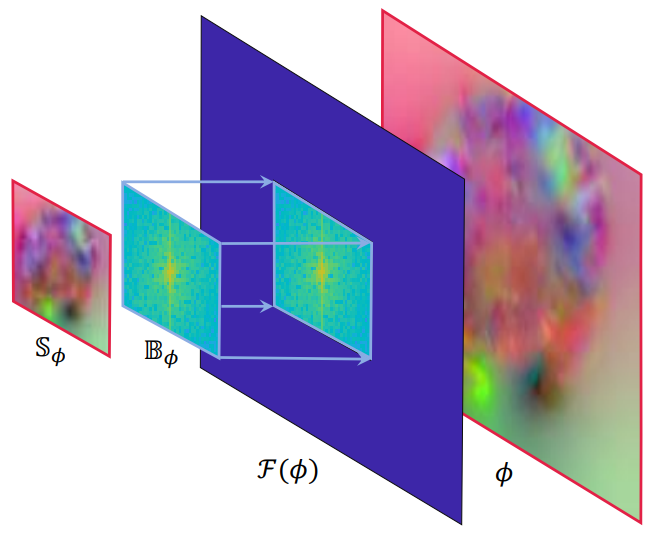
\includegraphics[width=.65\linewidth]{DecoderDisplacementField.png} 
	\caption{Reconstruction of the displacement field via the decoder taken from~\cite{Fourier-Net+}.}
	\label{fig:DecoderDisplacementField}
\end{figure} 

\subsection{Diffeomorphic Transforms}
Diffeomorphic deformations are differentiable and invertible, thus preserving topology, which is a desirable property for transformations. $\phi: \mathbb{R}^N \rightarrow \mathbb{R}^N$ represents the deformation that maps the coordinates from one image to coordinates in another image, as long as both images have the dimension $N$. When using a stationary velocity field representation like e.g. \emph{DARTEL}~\cite{DARTEL}, the deformation field is defined through the following ordinary differential equation (ODE)~\cite{Dalca2018}:
\begin{equation}
	\frac{\partial \phi^{(t)}}{\partial t} = v(\phi^{(t)}),
\end{equation}
where $\phi^{(0)} = \text{Id}$ is the identity transformation and $t$ is time. The final registration field $\phi^{(1)}$ can be obtained by integrating the stationary velocity field $v$ over $t = [0, 1]$. This is typically done by integration numerically using scaling and squaring~\cite{ScaleAndSquare}. The integration of a stationary ODE represents a one-parameter subgroup of diffeomorphisms. In group theory, $v$ is a member of the Lie algebra and is exponentiated to produce $\text{exp}(v) = \phi^{(1)}$, which is also a member of the Lie group. From the properties of one-parameter subgroups, for any scalars $t$ and $t'$, $\text{exp}((t + t') \cdot v) = \text{exp}(t \cdot v) \circ \text{exp}(t' \cdot v)$, where $\circ$ is a composition map associated with the Lie group. Starting from $\phi^{({1/2}^T)} = p + v(p)$ where $p$ is a map of spatial locations, we use the recurrence $\phi^{({1/2})^{t−1}} = \phi^{({1/2}^t)} \circ \phi^{({1/2}^t)}$ to obtain $\phi^1 = \phi^{(1/2)} \circ \phi^{(1/2)}$. $T$ is chosen so that $v \approx 0$~\cite{Dalca2018}. \\
As diffeomorphic deformations are defined as smooth and invertible deformations, the output of the iDFT layer in \emph{Fourier-Net} can be regarded as a stationary velocity field $v$ instead of a displacement field $\phi$. In Figure~\ref{fig:Fourier-Net} scaling and squaring layers are visualized. These apply the diffeomorphic transformation in three steps~\cite{ScaleAndSquare}:
\begin{enumerate}
	\item Scaling: Divide the velocity field $v$ by a factor $2^N$ , so that $\frac{v}{2^N}$ is close to zero (depending on the desired accuracy).
	\item Exponentiation: Compute $\text{exp}\big(\frac{v}{2^N}\big) = \phi^{(1)}\big(\frac{v}{2^N}\big)$ with a first-order explicit numerical scheme.
	\item Squaring: $N$ recursive squarings of $\phi^{(1)}\big(\frac{1}{2^N}\big) = \text{exp}\big(\frac{v}{2^N}\big)$ to yield an accurate estimation of $\phi^{(1)}(1) = \phi^{(1)}\big(\frac{1}{2^N}\big)^{2^N} = \text{exp}\big(\frac{v}{2^N}\big)^{2^N} = \text{exp}(v)$.
\end{enumerate}
Thus, the diffeomorphic deformation can be efficiently calculated. When used, the specific version is then called \emph{Fourier-Net Diff} to differentiate it from the baseline version.




\subsection{Spatial Transformer}
The warping layer of \emph{Fourier-Net} utilizes the \emph{Spatial Transformer}~\cite{SpatialTransformer}, which allows for spatial image manipulation within the network. This is a differentiable and learnable module for neural networks which applies a spatial transformation to a feature map during a single forward pass. The spatial transformer mechanism is split into three parts as seen in Figure~\ref{fig:SpatialTransformer}. First is the localization network, which takes the input and outputs the parameters for the transformation. These are then used to create a sample grid using the grid generator. Lastly, the sampler produces the output feature map based on the input at the grid points.\\
From the input feature map $U \in \mathbb{R}^{H \times W \times C}$ with width $W$, height $H$ and channels $C$ the localization network $f_{\text{loc}}$ computes the parameters $\theta = f_{\text{loc}}(U)$ of the transformation $\mathcal{T}_\theta$ which is later applied to the feature map. Thus the size of $\theta$ varies depending on the transformation. 
%(e.g. 6D for an affine transformation). 
The localization network function can both be implemented as a fully-connected network or as a CNN, but should include a final regression layer to produce the transformation parameters.\\
In order to warp the input feature map, each output pixel is computed by applying a sampling kernel centered at a particular location in the input feature map. The output pixels are defined to lie on a regular grid $G = {G_i}$ of pixels, forming an output feature map $V \in \mathbb{R}^{H' \times W' \times C}$, where $H'$ and $W'$ are the height and width of the grid with C again being the number of channels, which is the same for input and output.\\
In order to perform a spatial transformation of the input feature map $U$, the sampler must take the set of sampling points $\mathcal{T}_\theta(G)$, along and produce the sampled output feature map $V$. Each coordinate $(x_i^s, y_i^s)$ in $\mathcal{T}_\theta(G)$ defines the spatial location in the input where a sampling kernel is applied to get the value at a particular pixel in the output:
\begin{equation}
	V_i^c = \sum^{H}_{n} \sum^{W}_{m} U_{nm}^c k(x_i^s - m; \Phi_x) k(y_i^s - n; \Phi_y),
\end{equation}
with $\Phi_x$ and $\Phi_y$ being the parameters for a generic sampling  kernel $k$ that defines the image interpolation, $U_{nm}^c$ is the value of the input feature maps at location $(n,m)$ in the channel $c \in [1, ..., C]$ and $V_i^c$ is the value for every pixel $i \in [1, ..., H'W']$ for the output feature map. Any sampling kernel can be used, as long as (sub-) gradients can be defined with respect to $(x_i^s, y_i^s)$ to allow the loss gradients to flow back not only to the input feature map, but also to the sampling grid coordinates and therefore back to the transformation parameters $\theta$ and localization network, thus enabling back-propagation~\cite{SpatialTransformer}.
\begin{figure}[htpb]
	\centering
	\graphicspath{{images/}{\main/images/}}
	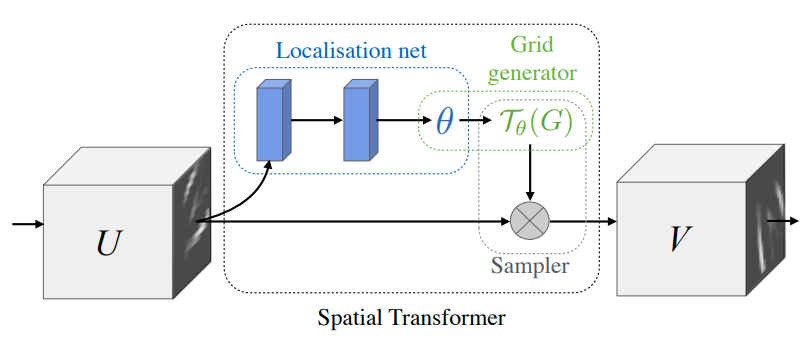
\includegraphics[width=\linewidth]{SpatialTransformer.png} 
	\caption{Architecture of the \emph{Spatial Transformer} taken from~\cite{SpatialTransformer}.}
	\label{fig:SpatialTransformer}
\end{figure}


\subsection{Loss Function}
The loss function consists of two parts to enable unsupervised learning, which are balanced using the scalar parameter $\lambda$. The first, $\mathcal{L}_{1}$, measures the similarity between the fixed image and the moving image after warping, while the second, $\mathcal{L}_{2}$, ensures a smooth displacement field. Thus, the unsupervised loss $\mathcal{L}$ can be calculated as follows:
\begin{equation}	\label{eq:unsupervisedLoss}
	\begin{split} 
		\mathcal{L}(\Theta) &= \min  \bigg( \mathcal{L}_{1} (\phi(\Theta))  + \lambda \cdot \mathcal{L}_{2} (\phi(\Theta)) \bigg) \\
		&= \min  \bigg( \mathcal{L}_{1} (v(\Theta))  + \lambda \cdot \mathcal{L}_{2} (v(\Theta)) \bigg),
	\end{split}
\end{equation}
for both displacement fields $\phi$ and velocity fields $v$. The first part of the loss function consists of:
\begin{equation} \label{eq:L1-LossDisp}
	\mathcal{L}_{1} (\phi(\Theta)) = \frac{1}{N} \sum^{N}_{i=1} \mathcal{L}_{Sim} (M_i \circ (\phi_i(\Theta) + \text{Id}) - F_i),
\end{equation}
where $\circ$ denotes the warping operation, $N$ the number of training pairs with moving images $M_i$ and fixed images $F_i$, $\Theta$ the network parameters, $\phi_i$ the displacement field, Id the identity grid. $\mathcal{L}_{Sim}$ determines the similarity between warped moving images and fixed images via MSE or NCC, and the second term of the unsupervised loss, $\mathcal{L}_{2}$, defines the smoothness regularization function that controls smoothness of the displacement fields:
\begin{equation} \label{eq:L2-LossDisp}
	\mathcal{L}_{2} (\phi(\Theta)) = \frac{1}{N} \sum^{N}_{i=1} || \nabla \phi_i(\Theta) ||^2_2,
\end{equation}
with $\nabla$ denoting the first order gradient and $|| \cdot ||_2^2$ denoting the squared $L_2$-Norm. \\
When using the squaring and scaling layers, thus making the deformation of the moving image diffeomorphic, the loss needs to be modified by replacing the displacement field $\theta$ with the velocity field $v$. Thus, both parts of the of the loss function need to be changed:
\begin{equation}	\label{eq:L1-LossVeloc}
	\mathcal{L}_{1} (v(\Theta)) = \frac{1}{N} \sum^{N}_{i=1} \mathcal{L}_{Sim} (M_i \circ Exp(v_i(\Theta) - F_i),
\end{equation}
\begin{equation} \label{eq:L2-LossVeloc}
	\mathcal{L}_{2} (v(\Theta)) = \frac{1}{N} \sum^{N}_{i=1} || \nabla v_i(\Theta) ||^2_2  \bigg .
\end{equation}

\subsection{Training on OASIS}
We first trained \emph{Fourier-Net} and \emph{Fourier-Net+} with the \emph{OASIS} dataset, as it was used in the original publication. \emph{Fourier-Net}/\emph{Fourier-Net+} can work with both 2D and 3D inputs, however the latter are harder to visualize. As the \emph{OASIS} dataset provides 3D volumes with annotations, 2D image data can be obtained by slicing the 3D volumes (see Figure~\ref{fig:OASIS} with matching labels for Dice-Score calculation. Thus we can easily visualize the training success of the 2D network by looking at the difference between images before and after registration in addition to the Dice-Score, which can also be calculated for 3D data. Examples for this can be seen in Figure~\ref{fig:DifferencesTrainingProgress} with two examples from different stages of the training process. Despite the example in Figure~\ref{fig:Training29600it} being the far harder example to align the network performs better than before (see Figure~\ref{fig:Training800it}) due to the training progress.

\begin{figure}[htpb]
	\centering
	\graphicspath{{images/}{\main/images/}}
	\begin{subfigure}{0.45\textwidth}
		\centering
    		\includegraphics[width=\textwidth]{results1.png}
    		\caption{Training progress after 800 iterations.}
    		\label{fig:Training800it}
	\end{subfigure}
	\hfill
	\begin{subfigure}{0.45\textwidth}
		\centering
    		\includegraphics[width=\textwidth]{results2.png}
    		\caption{Training progress after 29600 iterations.}
    		\label{fig:Training29600it}
	\end{subfigure}
	\caption{Differences between moving and fixed images before and after registration.}
	\label{fig:DifferencesTrainingProgress}
\end{figure}

\subsection{Training on CMRxRecon}
For the further experiments we used the \emph{CMRxRecon} dataset. We reconstructed 2D images and trained the network similar to the \emph{OASIS} dataset.

\section{Fourier Net+}
\emph{Fourier-Net+}, as the name suggests, is an extension of Fourier-Net which takes the band-limited spatial representation of the images as input, instead of their original full-resolution counterparts. This leads to further reduction in the number of convolutional layers in the contracting path of the network, resulting in a decrease of parameters, memory usage, and computational operations. This makes \emph{Fourier-Net+} even more efficient than its predecessor~\cite{Fourier-Net+}.\\
As seen in Figure~\ref{fig:Fourier-Net+}, the network architecture is almost the same as for \emph{Fourier-Net} (see Figure~\ref{fig:Fourier-Net} for comparison). However, while the decoder, and thus the loss function, remain the same, the encoder is slightly altered to make the network even more efficient. For this, similarly to the decoder, a DFT is used, however this time the idea is applied to the input images. These are first transformed into the Fourier domain, then low-pass filtered by center-cropping and finally reconstructed from their band-limited representation back into the spatial domain via an iDFT. The two images, now compressed, are the input for the encoder of \emph{Fourier-Net}, meaning the CNN and following DFT. However, due to the band-limiting before the CNN, the latter can be made much more light-weight, thus reducing computational cost. This is visualized in Figure~\ref{fig:Fourier-Net+CNN}. Thus, \emph{Fourier-Net+} too is overall lighter than the baseline \emph{Fourier-Net} in terms of the number of parameters and computations. However, such a light network may face limitations in accurately capturing complex deformations. To counter this potential weakness, the authors propose a cascaded version of \emph{Fourier-Net+}, which uses multiple versions of \emph{Fourier-Net+} cascaded one after the other to achieve a better overall displacement field~\cite{Fourier-Net+}. A schematic for this can be seen in Figure~\ref{fig:Fourier-Net+Cascaded}.

\begin{figure}[htpb]
	\centering
	\graphicspath{{images/}{\main/images/}}
	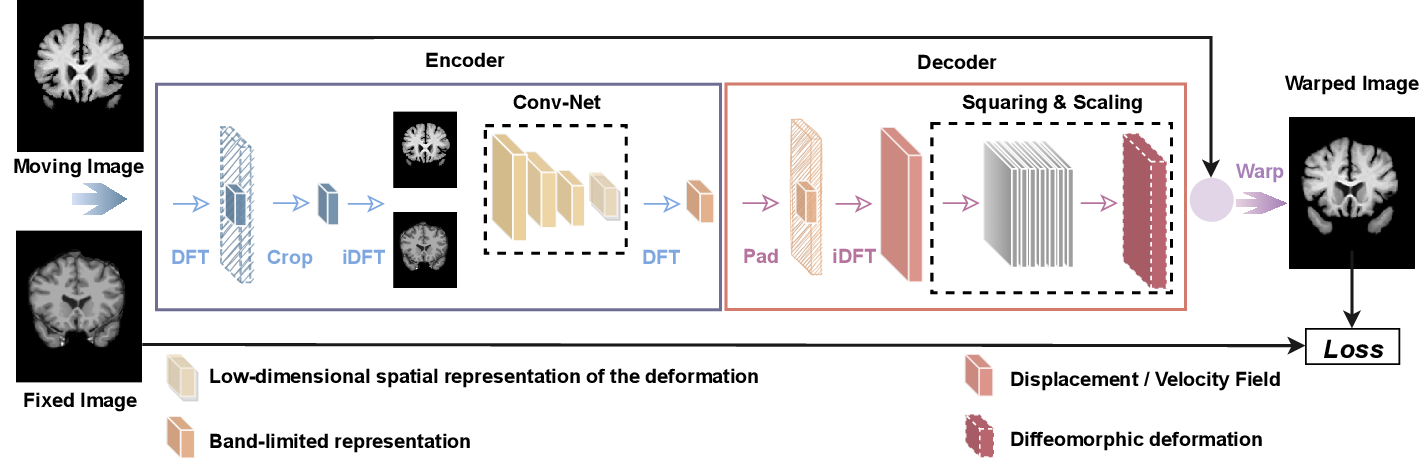
\includegraphics[width=\linewidth]{ArchitectureFourier-Net+.png} 
	\caption{Architecture of \emph{Fourier-Net+} taken from~\cite{Fourier-Net+}.}
	\label{fig:Fourier-Net+}
\end{figure}

\subsection{Changes to the Encoder}
In order to further reduce the amount of computational operations, \emph{Fourier-Net+} discards the early layers of the encoder. Instead, a DFT $\mathcal{F}(I_M)$ followed by a center-crop to produce the band-limited representation $\mathbb{B}_{I_M}$ in the frequency domain and iDFT are used to get the spatial patch $\mathbb{S}_{I_M}$, while the rest of the encoder from \emph{Fourier-Net} stays the same. The input $I_M$ is thus compressed to a lower resolution (i.e. band-limited) using the frequency space, which reduces the computational cost. This process is visualized in Figure~\ref{fig:Fourier-Net+EncoderCompression}. The encoder of \emph{Fourier-Net+} has several convolutional layers less in the contracting path compared to \emph{Fourier-Net}, which leads to a further accelerated registration process while reducing the memory footprint. These advantages are visualized in Figure~\ref{fig:Fourier-Net+CNN} where the amount of different layers between a conventional \emph{U-Net}, \emph{Fourier-Net} (with the smaller decoder) and \emph{Fourier-Net+} (with a smaller encoder and decoder) are shown.
\begin{figure}[htpb]
	\centering
	\graphicspath{{images/}{\main/images/}}
	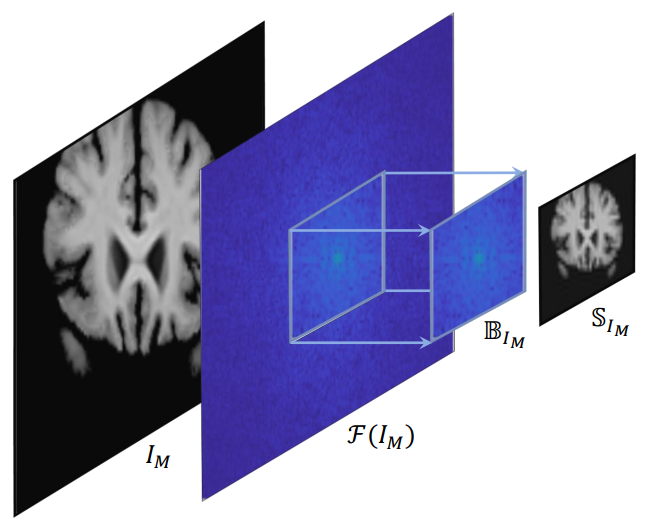
\includegraphics[width=.5\linewidth]{CompressionEncoder.png} 
	\caption{Compression in the frequency domain of the encoder used in \emph{Fourier-Net+} taken from~\cite{Fourier-Net+}.}
	\label{fig:Fourier-Net+EncoderCompression}
\end{figure}
\begin{figure}[htpb]
	\centering
	\graphicspath{{images/}{\main/images/}}
	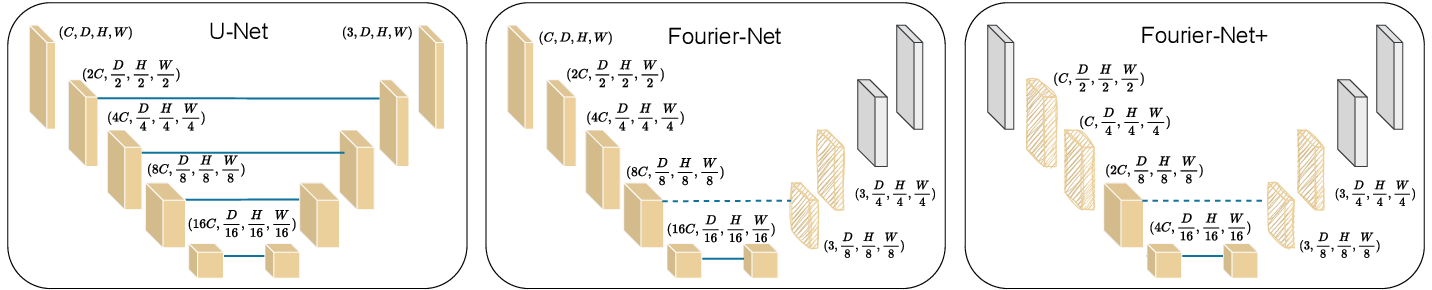
\includegraphics[width=\linewidth]{ArchitectureFourier-Net+CNN.png} 
	\caption{Architecture of the CNN for a typical U-Net, \emph{Fourier-Net} and \emph{Fourier-Net+} taken from~\cite{Fourier-Net+}.}
	\label{fig:Fourier-Net+CNN}
\end{figure}

\subsection{Effects of Cascading}
Why use cascaded version of the network?

\begin{figure}[htpb]
	\centering
	\graphicspath{{images/}{\main/images/}}
	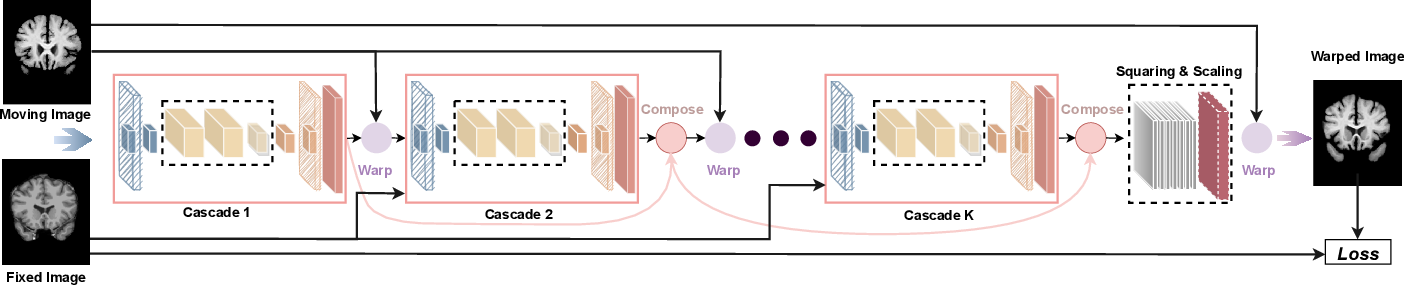
\includegraphics[width=\linewidth]{ArchitectureFourier-Net+Cascaded.png} 
	\caption{Cascaded version of \emph{Fourier-Net+} taken from~\cite{Fourier-Net+}.}
	\label{fig:Fourier-Net+Cascaded}
\end{figure}

\chapter{Experiments} %Evaluation
Describe the experiment and evaluation methods being used.
%Describe data here?!?


%%%%%%%%%%%%%%%%%%%%%%%%%%%%
%% Results and Discussion %%
%%%%%%%%%%%%%%%%%%%%%%%%%%%%

\chapter{Results and Discussion}
Here go the results with the discussion.


%%%%%%%%%%%%%%%%%%%%%%%
%%%%%  Conclusion %%%%%
%%%%%%%%%%%%%%%%%%%%%%%

\chapter{Conclusion}
Summery of all stuff...

\end{document}
